\chapter{Statistisk inferens} \label{ch:statistisk_inferens}
\textit{Da klassisk inferens ikke kan anvendes på adaptive procedurer, eftersom udvælgelsen af variable afhænger af data, introducerer vi i dette kapitel teori for inferens af lasso. Kapitlet er baseret på \citep{lockhart}, \citep{post_inference} samt kapitel 6 i \citep{hastie}.} \\[4mm]
%
Foruden bootstrap vil vi i den empiriske del betragte kovarians testen samt TG testen.
Kovarians testen anvendes for LARS algoritmen med lasso modifikation, mens TG testen anvendes for LARS algoritmen uden lasso modifikation og lasso modellen med en fast værdi af tuning parameteren.
Teorien for dette er udviklet i nyere tid og er stadig under udvikling.
\Rlang-pakkerne \texttt{covTest} og \texttt{selectiveInference} understøtter testene, som beskrives i dette kapitel.

\section{Kovarians testen} \label{subsec:kovarians_test}
I dette afsnit introduceres en test, der kan tildele \(p\)-værdier til prædiktorerne, som er udvalgt af lasso.
Testen er baseret på LARS algoritmen og blev introduceret i \citep{lockhart}.

Betragt det velkendte lineære regressionssetup
\begin{align}
\y = \X \tbeta + \boldsymbol{\epsilon}, \quad \boldsymbol{\epsilon} \sim N\del{\mathbf{0}, \sigma^2 \mathbf{I}_n}, \label{eq:set-up}
\end{align}
hvor \(\y\) er en \(n \times 1\) vektor med responsvariablen, \(\X\) er en \(n \times p\) matrix med prædiktorer og \(\tbeta\) er en \(p \times 1\) vektor, som skal estimeres.

Vi antager, at søjlerne i \(\X\) er i generel position, for at sikre at løsningsstien for LARS algoritmen med lasso modifikationen er entydig (se definition \ref{defn:general_position}).
Vi ønsker, at teste om prædiktoren, som tilføjes til den aktive mængde i step \(k\), er signifikant.
Den aktive mængde betegner somsagt prædiktorerne med ikke-nul koefficienter, og igen lader vi \(\lambda_k\) betegne \(k\)'te step i løsningsstien.
Lad \(\A_{k-1}\) betegne den aktive mængde i step \(k-1\) inden prædiktoren tilføjes, og lad \(\tilde{\tbeta}^\text{lasso}_{\A_{k-1}} \del{\lambda_{k+1}}\) være løsningen i \(\lambda_{k+1}\) ved kun at anvende prædiktorerne i \(\A_{k-1}\).
Denne løsning er eksplicit givet ved 
\begin{align*}
\tilde{\tbeta}^\text{lasso}_{\A_{k-1}} \del{\lambda_{k+1}} = \argmin_{\tbeta_{\A_{k-1}} \in \R^{\vert \A_{k-1} \vert}} \cbr{\frac{1}{2} \left\Vert \y - \X_{\A_{k-1}} \tbeta_{\A_{k-1}} \right\Vert_2^2 + \lambda_{k+1} \left\Vert \tbeta_{\A_{k-1}} \right\Vert_1},
\end{align*}
hvor \(\X_{\A_{k-1}}\) er en matrix, der består af søjlerne i \(\X\), som svarer til prædiktorerne i \(\A_{k-1}\).
Lad \(\widehat{\tbeta}^\text{lasso} \del{\lambda_{k+1}}\) betegne løsningen i \(\lambda_{k+1}\) udfra prædiktorerne \(\A_{k-1} \cup \cbr{j}\).
Da kan vi definere teststørrelsen af kovarians testen
\begin{align}
T_k^\text{cov} = \frac{1}{\sigma^2} \del{ \left\langle \y, \X \widehat{\tbeta}^\text{lasso} \del{\lambda_{k+1}} \right\rangle - \left\langle  \y, \X_{\A_{k-1}} \tilde{\tbeta}^\text{lasso}_{\mathcal{A}_{k-1}} \del{\lambda_{k+1}} \right\rangle}. \label{eq:6.5}
\end{align}
Intuitivt er teststørrelsen af kovarians testen i \eqref{eq:6.5} en funktion af differensen mellem \(\X \widehat{\tbeta}^\text{lasso}\) og \(\X_{\A_{k-1}} \tilde{\tbeta}^\text{lasso}_{\A_{k-1}}\), dvs de fittede værdier givet ved at inkludere og undlade \(j\)'te prædiktor i den nuværende aktive mængde.
Navnet af testen kommer af, at tælleren i \eqref{eq:6.5} kan betragtes som differensen mellem empiriske (ikke-centreret) kovarianser og et lille led. 
\footnote{Lad \(\y = \y - \tmu + \tmu\) med \(\tmu = \X \tbeta^*\), da kan tælleren af \eqref{eq:6.5} omskrives \(T_k^\text{cov} = \left\langle \y - \tmu, \X \widehat{\tbeta} \del{\lambda_{k+1}} \right\rangle - \left\langle \y - \tmu, \X_{\A_{k-1}} \tilde{\tbeta}_{\A_{k-1}} \del{\lambda_{k+1}} \right\rangle + \left\langle \tmu, \X \widehat{\tbeta} \del{\lambda_{k+1}} - \X_{\A_{k-1}} \tilde{\tbeta}_{\A_{k-1}} \del{\lambda_{k+1}} \right\rangle\).
De første to led er empiriske kovarianser og det sidste led er typisk lille.}
Desto større kovarians af \(\y\) og \(\X \widehat{\tbeta}^\text{lasso}\) sammenlignet med \(\X_{\A_{k-1}} \tilde{\tbeta}^\text{lasso}_{\A_{k-1}}\), desto vigtigere er \(j\)'te prædiktor i modellen \(\A_{k-1} \cup \cbr{j}\).
%Kovarians teststørrelsen evalueres i næste knot \(\lambda_{k+1}\), da \(j\)'te koefficient stadig er lig nul i \(\lambda_k\).
%I \(\lambda = \lambda_{k+1}\), ses den ...
% og dermed
%\begin{align*}
%\X \hat{\beta} \del{\lambda_k} = \X_{\A_{k-1}} \hat{\beta}_{\A_{k-1}} \del{\lambda_k} = \X_{\A_{k-1}} \tilde{\beta}_{\A_{k-1}} \del{\lambda_k}
%\end{align*}
%Det naturlig valg for tuning parameteren i \eqref{eq:6.5} er derfor \(\lambda= \lambda_{k+1}\).

Under nulhypotesen at lasso modellen med den aktive mængde \(\A_{k-1}\) indeholder alle sande aktive variable, dvs \(\hyp_0: \mathcal{A}_{k-1} \supseteq \text{supp} \del{\tbeta^*}\) (se definition \ref{defn:supp}), hvor \(\tbeta^*\) er den sande koefficientvektor, da har teststørrelsen i \eqref{eq:6.5} en asymptotisk standard eksponentiel fordeling
\begin{align*}
T_k^\text{cov} \overset{d}{\rightarrow} \text{Exp}\del{1}.
\end{align*}
Vi henviser til s. 425-441 i \citep{lockhart}, hvor resultatet bevises. 
Hvis \(\sigma^2\) er ukendt, kan den estimeres under den fulde model \(\widehat{\sigma}^2 = \frac{1}{n-p} \text{SSR}_p\). 
Dette indsættes i \eqref{eq:6.5}, og eksponential testen bliver en eksakt \(F_{2,n-p}\) test. \\
%
\begin{eks} \\
For diabetes data ønsker vi at udregne \(p\)-værdien for prædiktoren \texttt{hdl}, som tilføjes til den aktive mængde i fjerde step af LARS algoritmen (se figur \ref{fig:diabetes_covTest}). 
Da skal vi udregne kovariansen i \(\lambda_4\)??, der er givet ved \(\left\langle \y, \X \widehat{\tbeta}^\text{lasso} \del{\lambda_4} \right\rangle\).
Herefter fjernes prædiktoren \texttt{hdl}, hvilket giver den aktive mængde \(\A_{3}\), vi refitter i \(\lambda_4\) og udregner igen kovariansen i \(\lambda_4\), der er givet ved \(\left\langle  \y, \X_{\A_{2}} \tilde{\tbeta}^\text{lasso}_{\mathcal{A}_{2}} \del{\lambda_{4}} \right\rangle\).
Teststørrelsen af kovarians testen er da givet ved
\begin{align*}
T_3^\text{cov} = \frac{1}{\sigma^2} \del{ \left\langle \y, \X \widehat{\tbeta}^\text{lasso} \del{\lambda_{4}} \right\rangle - \left\langle  \y, \X_{\A_{2}} \tilde{\tbeta}^\text{lasso}_{\mathcal{A}_{2}} \del{\lambda_{4}} \right\rangle}.
\end{align*}
%
\begin{figure}[H]
\centering
\scalebox{0.6}{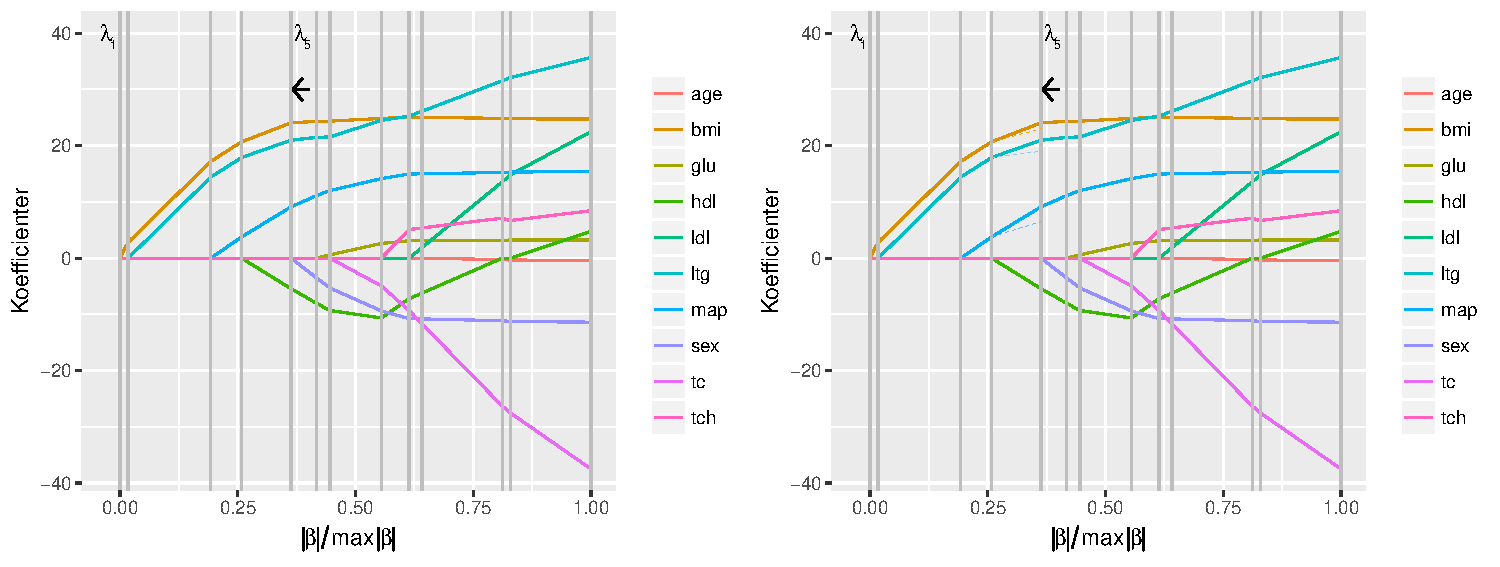
\includegraphics{fig/img/diabetes_covTest.pdf}}
\caption{Illustration af kovarians testen for prædiktoren \texttt{hdl}.} \label{fig:diabetes_covTest}
\end{figure}
%
Resultatet af kovarians testen anvendt på diabetes data er givet i tabel \ref{tab:diabetes_covTest}.
Nulhypotesen afvises for \texttt{bmi}, \texttt{ltg}, \texttt{map} og \texttt{hdl} som tilføjes til den aktive mængde i step 1-4, hvilket betyder, at disse prædiktorer er signifikante.
For de resterende prædiktorer kan nulhypotesen ikke afvises.
%
\begin{table}[ht] 
\centering 
\begin{tabular}{lccc}
%\multicolumn{3}{l}{LARS algoritmen med lasso modifikation} \\
\toprule
Prædiktor & Cov test & \(p\)-værdi \\
\midrule
\texttt{bmi} & 9.0612 & 0.0000 \\
\texttt{ltg} &50.9187 & 0.0000 \\
 \texttt{map}     &       5.5886 & 0.0040 \\
 \texttt{hdl}      &    5.9933 & 0.0027 \\
\texttt{sex}     &   4.8039 & 0.0086 \\
\texttt{glu}     &  0.1593 & 0.8528 \\
\texttt{tc}  &         3.2848 & 0.0384 \\
\texttt{tch}    &        0.6153 & 0.5409 \\
\texttt{ltg}    &        0.1639 & 0.8489 \\
\texttt{age} &       0.0150 & 0.9851 \\ \bottomrule
\end{tabular}
\caption{Kovarians testen for LARS algoritmen med lasso modifikation for diabetes data. Vi har, at \(\widehat{\sigma}^2 = 54.0975\) og nulfordelingen \(F_{2,432}\).} \label{tab:diabetes_covTest}
\end{table} 
\end{eks}

Kovarians testen er det naturlige analog til resultaterne for frihedsgrader for lasso og LARS.
Som nævnt tidligere har lasso med \(k\) ikke-nul koefficienter \(k\) frihedsgrader, mens LARS anvender en frihedsgrad for hvert step.
Kovarians testen har middelværdi lig en, som er antallet af frihedsgrader per step.
Hermed kan man sige at Exp\(\del{1}\) fordelingen svarer til \(\chi_1^2\) fordelingen for adaptive procedurer.

%Kovarians testen har nogle begrænsninger.
%Først skal der gælde, at kolonner af \(\X\) er i generel position.
%%Hvis der eksisterer en kategorisk variabel blandt prædiktorerne, og den resulterende variabel beskrives af dummy variable, da er antagelse om at kolonnerne af \(\X\) er i general position altså ikke overholdt.
%Derudover tager testen ikke højde for, hvis nogle variable medtages i modellen mere end én gang (som er tilladt for lasso modifikationen af LARS algoritmen), da behandles hver situation separat og testene udføres separat.
%Til sidst er testen kun asymptotisk.
%
%I næste afsnit introduceres en test som kan anvendes efter modeludvælgelse og som giver en eksakt fordeling af teststørrelsen.
\section{Post-selection inferens}
Klassisk statistisk inferens kan ikke anvendes for adaptive procedurer.
I dette afsnit beskrives teste til inferens efter variabeludvælgelse med en adaptiv metode.
Teorien omkring post-selection inferens er udviklet i nyere tid og er stadig under udvikling.
R-pakkerne \texttt{covTest} og \texttt{selectiveInference} understøtter testene som beskrives i dette afsnit.

\subsection{Kovarians test} \label{subsec:kovarians_test}
I dette afsnit introduceres en test, der tildeler \(p\)-værdier til prædiktorerne valgt af adaptive metoder.
Testen er baseret på LARS algoritmen og blev introduceret af \citep{lockhart}.

Betragt det velkendte lineær regression setup med en responsvariable \(\y \in \mathbb{R}^n\) og en matrix af prædiktorer \(\X \in \mathbb{R}^{n \times p}\), som er relateret ved
\begin{align*}
\y = \X \beta + \boldsymbol{\epsilon}, \quad \boldsymbol{\epsilon} \sim N\del{\mathbf{0}, \sigma^2 \mathbf{I}},
\end{align*}
hvor \(\beta \in \mathbb{R}^p\) er ukendte koefficienter, som skal estimeres.

For at motivere kovarians testen, vil vi først betragte forward-stepwise regression.
Proceduren udvælger én prædiktor af gangen og vælger den prædiktor således at summen af kvadrerede residualer aftager mest.
Lad \(\text{SSR}_k\) betegne summen af kvadrerede residualer for modellen med \(k\) prædiktorer.
Da kan vi udlede en teststørrelse ved at betragte ændringen i SSR
\begin{align*}
R_k = \frac{1}{\sigma^2} \del{\text{SSR}_{k-1} - \text{SSR}_k},
\end{align*}
hvor \(\sigma\) antages at være kendt. 
Denne teststørrelse følger en \(\chi_1^2\) fordeling.
Hvis \(\sigma\) ikke er kendt, da den estimeres udfra sample variansen, hvilket resulterer i en \(F\)-test eller ækvivalent en \(t\)-test til at teste om variabel \(j\) er signifikant.

Betragt forward stepwise regression: start med en tom model, tilføj en prædiktor af gangen, for hvert step vælg den prædiktor \(j\) som giver den største fald i SSR.
Figur \ref{fig:covarians_test}(a) viser kvantilerne for \(R_1\) af forward stepwise regression imod en \(\chi_1^2\) fordeling, hvor \(\beta=0\).
 

%
\begin{figure}[H]
\centering
 \scalebox{0.5}{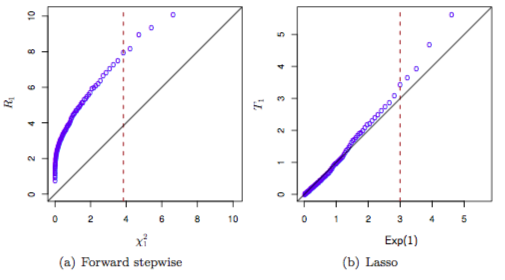
\includegraphics{fig/covarians_test.jpg}}
\caption{Et .}
\label{fig:covarians_test}
\end{figure}
%

Inden vi giver en formel beskrivelse af kovarians testen, gives en betingelse for model matricen \(\X\).
\begin{defn}
Kolonnerne \(\mathbf{X}_1, \ldots, \mathbf{X}_p\) siges at være i generel position hvis the affine span af enhver \(k+1\) vektorer \(s_1 \X_1, \ldots, s_{k+1} \X_{k+1}\) ikke indeholder ethvert element af mængden \(\cbr{\pm \X_i : \ i \neq i_1, \ldots, i_{k+1}}\) for ethvert fortegn \(s_1, \ldots, s_{k+1} \in \cbr{-1,1}\), for \(k < \min \cbr{n,p}\). 
\end{defn}
Ovenstående betingelse er svag og gælder blandt andet når indgangene af \(\X\) kommer af en kontinuert sandsynligheds fordeling.
At kolonnerne af model matrix er i generel position sikre at lasso stien er entydig, som vises i ---.

Herefter kan vi defineres teststørrelse af kovarians testen og forklare hvordan \(p\)-værdierne findes.




Lad $\lambda_1 > \lambda_2 > \ldots > \lambda_K$ være knuderne returneret af LARS algoritmen.
Disse er værdierne af regularitets parameteren $\lambda$ ,hvor der sker en ændring i mængden af aktive prædiktorer.
V ønsker, at teste om prædiktoren valgt i \(\lambda_k\) af LARS algoritmen er signifikant.
Lad \(\mathcal{A}_{k-1}\) være den aktive mængde, som består af prædiktorerne med ikke-nul koefficienter, inden denne prædiktor er tilføjet og lad estimatet til slut af dette step være \(\hat{\beta} \del{\lambda_{k+1}}\).
Lad \(\hat{\beta}_{\mathcal{A}_{k-1}} \del{\lambda_{k+1}}\) være løsningen af lasso problemet ved blot at anvende prædiktorerne  i \(\mathcal{A}_{k-1}\), i \(\lambda=\lambda_{k+1}\).
Kovarians teststørrelsen er da defineret ved
\begin{align}
T_k^\text{cov} = \frac{1}{\sigma^2} \del{ \left\langle \y, \X \hat{\beta} \del{\lambda_{k+1}} \right\rangle - \left\langle  \y, \X \hat{\beta}_{\mathcal{A}_{k-1}} \del{\lambda_{k+1}} \right\rangle}. \label{eq:6.5}
\end{align}
Teststørrelsen måler hvor stor en andel af kovariansen mellem outcome og den fittede model som kan tilskrives prediktoren som netop er tilføjet til modellen, dvs forbedringen over intervallet \(\del{\lambda_k, \lambda_{k+1}}\).

Under nulhypotesen at alle $k-1$ variable er i modellen, og under generelle betingelser for modelmatricen $\X$, gælder der for prediktoren i næste trin at
\begin{align*}
T_k^\text{cov} \overset{d}{\rightarrow} \text{Exp}\del{1}
\end{align*}
når \(n, p \rightarrow \infty\).
Når \(\sigma^2\) er ukendt, kan den estimeres under den fulde model \(\hat{\sigma}^2 = \frac{1}{n-p} \text{RSS}_p\). 
Dette indsættes i \eqref{eq:6.5}, og eksponential testen bliver en eksakt \(F_{2,n-p}\) test.

Denne test er også det naturlige analog til degrees of freedom resultaterne for lasso \eqref{eq:df_lasso} og LARS (section 2.5).
Lasso med \(k\) ikke-nul koefficienter forventes at have \(k\) frihedsgrader, og LARS anvender en frihedsgrad for hver segment \(\del{\lambda_{k+1}, \lambda_k}\) langs stien.
Kovarians testen har middelværdi lig en, som er antal frihedsgrader per trin.


Hvis \(\X\) er ortogonal, da er teststørrelsen for kovarians testen givet ved
\begin{align*}
T_k^\text{cov} = \frac{1}{\sigma^2} \lambda_k \del{\lambda_k - \lambda_{k+1}}
\end{align*} 
Derudover fandt vi at \eqref{eq:ortogonal_lasso} som også kan skrives \(\hat{\beta}_j = S_\lambda \del{\frac{1}{n} \mathbf{x}_j^T \y}\).
Lad \(\mathbf{U}_j = \mathbf{x}_j^T \y\) for \(j=1,\ldots, p\). 
Knots i lasso stien er blot værdierne af \(\lambda\) for hvilket koefficienterne er ikke-nul
\begin{align*}
\lambda_1 = \vert \mathbf{U}_{(1)} \vert, \quad \lambda_2 = \vert \mathbf{U}_{(2)} \vert, \quad \ldots, \lambda_p = \vert \mathbf{U}_{(p)} \vert, \quad,
\end{align*}
hvor \(\vert \mathbf{U}_{(1)} \vert \geq \vert \mathbf{U}_{(2)} \vert \geq \dots \geq \vert \mathbf{U}_{(p)} \vert\) er order statistics af \(\vert \mathbf{U}_1 \vert, \ldots, \vert \mathbf{U}_p \vert\).
Derfor 
\begin{align*}
T_k^\text{cov} = \frac{1}{\sigma^2}  \vert \mathbf{U}_{(k)} \vert \del{ \vert \mathbf{U}_{(k)} \vert -  \vert \mathbf{U}_{(k+1)} \vert}
\end{align*}


Kovarians testen har nogle begrænsninger.
Først skal der gælde en betingelse for model matricen \(\X\).
Hvis der eksisterer en kategorisk variabel blandt prædiktorerne, og den resulterende variabel beskrives af dummy variable, da er antagelse om at kolonnerne af \(\X\) er i general position altså ikke overholdt.
Derudover tager testen ikke højde for, hvis nogle variable medtages i modellen mere end én gang (som er tilladt for lasso modificeringen af LARS algoritmen), da behandles hver situation separat og testene udføres separat.
Til sidst er testen kun asymptotisk.

I næste afsnit introduceres en test som kan anvendes efter modeludvælgelse og som giver en eksakt fordeling af teststørrelsen.

\newpage
\subsection{Teste baseret på polyhedral lemmaet}
\citep{post_inference}


I dette afsnit introduceres teste der er baseret på polyhedral lemmaet.
Testene er \textit{TG test} og \textit{spacing test}. 
Disse kan håndterer enhver procedure for hvilket udvægelsen kan karakteriseres ved en mængde af lineære uligheder i \(\y\).
Med andre ord kan udvægelsen skrives som \(\cbr{\mathbf{A} \y \leq b}\) for en matrix \(\mathbf{A}\) og vektor \(b\).
Den kan anvendes til trinene af LARS algoritmen, hvor det giver en eksakt form af kovarians testen.

Antag \(\y \sim N\del{\boldsymbol{\mu}, \sigma^2 \mathbf{I}_{n \times n}}\) og at vi ønsker at lave inferens betinget på hændelsen \(\cbr{\mathbf{A} \y \leq b}\).
Mere præcis ønsker vi at lave inferens om \(\boldsymbol{\eta}^T \boldsymbol{\mu}\), hvor \(\boldsymbol{\eta}\) muligvis afhænger af udvægelsen.
Hvis lasso, LARS .. har udvalgt denne mængde, da kan vi udføre inferens  af de udvalgte variable.
Vi kunne eventuelt være interesseret i regressions koefficienterne af \(\y\) på \(\X_\mathcal{A}\), dvs \(\hat{\theta}= \del{\X_\mathcal{A}^T \X_\mathcal{A}}^{-1} \X_\mathcal{A}^T \y\).
Disse svarer til populations parametrene \(\theta= \del{\X_\mathcal{A}^T \X_\mathcal{A}}^{-1} \X_\mathcal{A}^T \boldsymbol{\mu}\), koefficienterne af projectionen af \(\boldsymbol{\mu}\) på \(\X_\mathcal{A}\).
Dermed kunne \(\boldsymbol{\eta}^T \boldsymbol{\mu}\) svarer til én af disse koefficienter, og dermed er \(\boldsymbol{\eta}\) en af kolonnerne af \(\X_\mathcal{A} \del{\X_\mathcal{A}^T \X_\mathcal{A}}^{-1}\). Dette eksempel fortsættes senere.


\subsubsection{Conditioning on a single polyhedron}
Antag \(\y \sim N \del{\boldsymbol{\mu}, \Sigma}\) og \(\boldsymbol{\eta} \in \mathbb{R}^n\) er en potential retning.
For at forstå fordelingen af
\begin{align*}
\boldsymbol{\eta}^T \y \given \cbr{ \mathbf{A} \y \leq b},
\end{align*}
kan vi omskrive \(\cbr{\mathbf{A} \y \leq b}\) udfra \(\boldsymbol{\eta}^T \y\) og en komponent \(\mathbf{z}\) som er uafhængig af \(\boldsymbol{\eta}^T \y\). Denne komponent er givet ved
\begin{align}
\mathbf{z} = \del{\mathbf{I} - \mathbf{c} \boldsymbol{\eta}^T} \y, \label{eq:z}
\end{align}
hvor 
\begin{align}
\mathbf{c} = \Sigma \boldsymbol{\eta} \del{\boldsymbol{\eta}^T \Sigma \boldsymbol{\eta}}^{-1}. \label{eq:c}
\end{align}
Det ses let, at \(\mathbf{z}\) er ukorreleret og dermed uafhængig af \(\boldsymbol{\eta}^T \y\).
Hvis \(\Sigma = \sigma^2 \mathbf{I}\), da er \(\mathbf{z}\) blot residualen \(\del{\mathbf{I} - P_{\boldsymbol{\eta}}} \y \) fra projektionen \(\y\) på \(\boldsymbol{\eta}\).
Vi kan nu omskrive \(\cbr{\mathbf{A} \y \leq b}\) udfra \(\boldsymbol{\eta}^T \y\) og \(\mathbf{z}\).
%
\begin{lem}[Polyhedral lemma] \label{lem:polyhedral}
Lad \(\mathbf{z}\) være defineret som i \eqref{eq:z} og \(\mathbf{c}\) som i \eqref{eq:c}. Da kan \(\cbr{\mathbf{A} \y \leq b}\) udfra \(\boldsymbol{\eta}^T \y\) omskrives til følgende:
\begin{align}
\cbr{\mathbf{A} \y \leq b} = \cbr{\mathcal{V}^- \del{\y} \leq \boldsymbol{\eta}^T \y \leq \mathcal{V}^+ \del{\y}, \mathcal{V}^0 \del{\y} \geq 0}, \label{eq:polyhedral}
\end{align}
hvor
\begin{align}
\mathcal{V}^- \del{\y} &= \max_{j: \alpha_j <0} \frac{b_j - \del{\mathbf{A} \y}_j + \alpha_j \boldsymbol{\eta}^T \y}{\alpha_j} \label{eq:V-} \\
\mathcal{V}^+ \del{\y} &= \min_{j: \alpha_j >0} \frac{b_j - \del{\mathbf{A} \y}_j + \alpha_j \boldsymbol{\eta}^T \y}{\alpha_j} \label{eq:V+} \\
\mathcal{V}^0 \del{\y} &= \min_{j: \alpha_j =0} \del{b_j - \del{\mathbf{A} \y}_j}.  \label{eq:V0} 
\end{align}
og \(\alpha=\frac{\mathbf{A} \boldsymbol{\eta}}{\Vert  \boldsymbol{\eta} \Vert_2^2}\).
Yderligere  er \(\boldsymbol{\eta}^T \y\) og \(\del{\mathcal{V}^-\del{\y}, \mathcal{V}^+\del{\y},\mathcal{V}^0\del{\y}}\) uafhængige. 
\end{lem}
\begin{proof}
Vi kan dekomponere \(\y = \mathbf{c} \del{\boldsymbol{\eta}^T \y} + \mathbf{z}\) og opskrive polyhedronet som følgende
\begin{align*}
\cbr{\mathbf{A} \y \leq b} &= \cbr{\mathbf{A} \del{\mathbf{c} \del{\boldsymbol{\eta}^T \y} + \mathbf{z}} \leq b} \\
&= \cbr{\mathbf{A} \mathbf{c} \del{\boldsymbol{\eta}^T \y} \leq b - \mathbf{A} \mathbf{z} } \\
&= \cbr{\del{\mathbf{A} \mathbf{c}}_j \del{\boldsymbol{\eta}^T \y} \leq b_j - \del{\mathbf{A} \mathbf{z}}_j \text{ for alle } j} \\
&= \begin{cases}
\boldsymbol{\eta}^T \y \leq \frac{b_j - \del{\mathbf{A} \mathbf{z}}_j}{\del{\mathbf{A} \mathbf{c}}_j}, \quad j:\del{\mathbf{A} \mathbf{c}}_j > 0 \\
\boldsymbol{\eta}^T \y \geq \frac{b_j - \del{\mathbf{A} \mathbf{z}}_j}{\del{\mathbf{A} \mathbf{c}}_j}, \quad j:\del{\mathbf{A} \mathbf{c}}_j < 0 \\
0 \leq b_j - \del{\mathbf{A} \mathbf{z}}_j, \quad j:\del{\mathbf{A} \mathbf{c}}_j = 0
\end{cases}.
\end{align*}
Da \(\boldsymbol{\eta}^T \y \) er den samme mængde for alle \(j\), må det mindste være maksimum af de nedre grænser, som er \(\mathcal{V}^- \del{\mathbf{z}}\), og ikke mere end minimum af de øvre grænser, som er \(\mathcal{V}^+ \del{\mathbf{z}}\).
\end{proof}
Resultatet i \eqref{eq:polyhedral} hvor \(\mathcal{V}^-\), \(\mathcal{V}^+\) og \(\mathcal{V}^0\) defineres i \eqref{eq:V-}-\eqref{eq:V0} er deterministisk og gælder for alle \(\y\).
Blot uafhængigheds resultatet afhænger af normaliteten af \(\y\).
Se figur \ref{fig:polyhedron} for en geometrisk illustration af lemmaet.
For simplicitet antages at \(\Sigma= \mathbf{I}\).
Lad os dekomponere \(\y=P_{\boldsymbol{\eta}} \y + P_{\boldsymbol{\eta}^\perp} \y\), hvor \(P_{\boldsymbol{\eta}} \y = \frac{\boldsymbol{\eta} \boldsymbol{\eta}^T \y}{\Vert \boldsymbol{\eta} \Vert_2^2}\) er projectionen af \(\y\) langs \(\boldsymbol{\eta}\) og  \(P_{\boldsymbol{\eta}^\perp} \y = \y - P_{\boldsymbol{\eta}} \y\) er projectionen på orthokomplement af \(\boldsymbol{\eta}\).
Vi kan betragte \(\y\) som afvigelse fra \(P_{\boldsymbol{\eta}^\perp} \y\) af en mængde \(\boldsymbol{\eta}^T \y\), langs linjen bestemt af \(\boldsymbol{\eta}\).
Mængderne \(\mathcal{V}^-\) og \(\mathcal{V}^+\) betegner hvor langt vi kan afvige fra hver side af \(P_{\boldsymbol{\eta}^\perp} \y\) inden \(\y\) forlader polyhedronen.
Dette giver anledning til uligheden \(\mathcal{V}^- \leq \boldsymbol{\eta}^T \y \leq \mathcal{V}^+\).
Some faces of polyhedronen kan være perfekt justeret med \(\boldsymbol{\eta}\), dvs deres normal vektorer og \(\boldsymbol{\eta}\) er ortogonale.
Dette kan tjekkes udfra \(\mathcal{V}^0\) ved at \(\y\) ligger på den rigtige side af these faces.  
--
Betinget \(P_{\boldsymbol{\eta}^\perp} \y\), ses at hændelsen \(\cbr{\mathbf{A} \y \leq b}\) er ækvivalent med hændelsen \(\mathcal{V}^- \del{\y} \leq \boldsymbol{\eta}^T \y \leq \mathcal{V}^+ \del{\y}\). Yderligere er \(\mathcal{V}^- \del{\y}\) og \(\mathcal{V}^+ \del{\y}\) uafhængige af \(\boldsymbol{\eta}^T \y\), da disse kun er funktioner af \(P_{\boldsymbol{\eta}^\perp} \y\), som er uafhængige af \(\y\).
--

Af lemma \ref{lem:polyhedral} kan fordelingen af enhver lineær funktion \(\boldsymbol{\eta}^T \y\) betinget \(\mathbf{A} \y \leq b\) skrives som følgende betinget fordeling
\begin{align*}
\boldsymbol{\eta}^T \y \given \mathcal{V}^- \del{\y} \leq \boldsymbol{\eta}^T \y \leq \mathcal{V}^+ \del{\y}, \mathcal{V}^0 \del{\y} \leq 0.
\end{align*}
Da \(\boldsymbol{\eta}^T \y\) er normalfordelt, er overstående truncated normalfordelt, dvs med stokastiske truncation grænser.

En simpel transformation fører tila pivotal statistic, som er kritisk for inferens af \(\boldsymbol{\eta}^T \theta\).

%
\begin{figure}[H]
\centering
\scalebox{1}{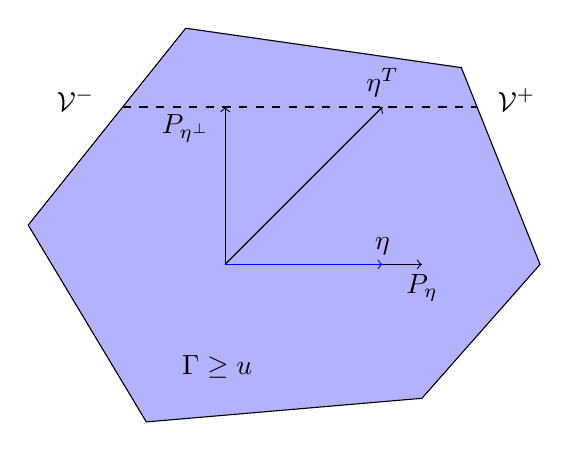
\begin{tikzpicture}
\draw (-1,-2) -- (-2.5,0.5) -- (-0.5,3)-- (3,2.5) -- (4,0) -- (2.5,-1.7) -- (-1,-2)[fill = blue!30];
\draw [<-] (0,2) node [label={[xshift=-0.5cm, yshift=-0.7cm]$P_{\boldsymbol{\eta}^\perp} \y$}] {} -- (0,0);
\draw[<-] (2.5,0) node [below] {$P_{\boldsymbol{\eta}} \y$} -- (0,0);
\draw[<-][blue] (2,0) node [black, above] {$\boldsymbol{\eta}$} -- (0,0);
\draw[<-] (2,2) node [above] {$\boldsymbol{\eta}^T \y$} -- (0,0) node [label={[xshift=1.7cm, yshift=1cm]$\y$}] {};
\draw[dashed] (-1.3,2) node [label={[xshift=-0.6cm, yshift=-0.3cm]$\mathcal{V}^- \del{\y}$}] {} -- (3.2,2) node [label={[xshift=0.5cm, yshift=-0.3cm]$\mathcal{V}^+ \del{\y}$}] {};
\draw node [label={[xshift=-0.1cm, yshift=-1.7cm]$\cbr{\Gamma \y \geq u}$}] {};
\end{tikzpicture}}
\caption{Geometrisk illustration af lemma \ref{lem:polyhedral} for \(n=2\) og \(\Vert \boldsymbol{\eta} \Vert_2=1\). 
Det blå område er udvælgelseshændelsen \(\cbr{\mathbf{A} \y \leq b}\)} \label{fig:polyhedron}
\end{figure}
%
\begin{lem}  \label{lem:lem2}
Lad \(\Phi \del{x}\) betegne fordelingsfunktionen af en standard normalfordeling, da er fordelingsfunktionen for en normalfordeling med middelværdi \(\mu\) og varians \(\sigma^2\) af en stokastisk variable indenfor intervallet \(\sbr{a,b}\) givet ved
\begin{align*}
F_{\mu, \sigma^2}^{\sbr{a,b}} \del{x} = \frac{\Phi\del{\frac{x-\mu}{\sigma}} - \Phi\del{\frac{a-\mu}{\sigma}}}{\Phi\del{\frac{b-\mu}{\sigma}} - \Phi\del{\frac{a-\mu}{\sigma}}}.
\end{align*}
For \(\boldsymbol{\eta}^T \Sigma \boldsymbol{\eta} \neq 0\) da er teststørrelsen \(F_{\boldsymbol{\eta}^T \theta, \boldsymbol{\eta}^T \Sigma \boldsymbol{\eta}}^{\sbr{\mathcal{V}^-,\mathcal{V}^+}} \del{\boldsymbol{\eta}^T \y} \) a pivotal quantity betinget \(\mathbf{A} \y \leq b\):
\begin{align*}
\mathbb{P} \del{F_{\boldsymbol{\eta}^T \theta, \boldsymbol{\eta}^T \Sigma \boldsymbol{\eta}}^{\sbr{\mathcal{V}^-,\mathcal{V}^+}} \del{\boldsymbol{\eta}^T \y} \leq \alpha \given \mathbf{A} \y \leq b} = \alpha, 
\end{align*}
for ethvert \(0 \leq \alpha \leq 1\), hvor \(\mathcal{V}^-\) og \(\mathcal{V}^+\) er defineret i \eqref{eq:V-} samt \eqref{eq:V+}. 
\end{lem}
%
Denne pivotal statistic i lemmaet fører til gyldige betinget \(p\)-værdier for at teste nulhypotesen \(H_0: \boldsymbol{\eta}^T \boldsymbol{\mu}=0\) og tilhørende betinget konfidensintervaller for \(\boldsymbol{\eta}^T \theta\).
Nedenfor betragtes en two-sided inferens.
%
\begin{lem} \label{lem:lem3}
Givet \(\boldsymbol{\eta}^T \Sigma \boldsymbol{\eta} \neq 0\), antag at vi vil teste
\begin{align*}
H_0: \boldsymbol{\eta}^T \theta=0 \quad \text{imod} \quad H_1: \boldsymbol{\eta}^T \theta \neq 0.
\end{align*}
Definer teststørrelsen
\begin{align}
T=2 \cdot \min\cbr{F_{0, \boldsymbol{\eta}^T \Sigma \boldsymbol{\eta}}^{\sbr{\mathcal{V}^-, \mathcal{V}^+}} \del{\boldsymbol{\eta}^T \y}, 1 - F_{0, \boldsymbol{\eta}^T \Sigma \boldsymbol{\eta}}^{\sbr{\mathcal{V}^-, \mathcal{V}^+}} \del{\boldsymbol{\eta}^T \y}}, \label{eq:post_1.18}
\end{align}
hvor fordelingsfunktionen af \(\boldsymbol{\eta}^T \y \sim N \del{0,  \boldsymbol{\eta}^T \Sigma \boldsymbol{\eta}}\) i intervallet \(\sbr{\mathcal{V}^-, \mathcal{V}^+}\) er givet i lemma \ref{lem:lem2}.
Da er \(T\) en gyldig \(p\)-værdi for \(H_0\) betinget \(\mathbf{A} \y \leq b\)
\begin{align*}
\mathbb{P}_{\boldsymbol{\eta}^T \theta=0} \del{T \leq \alpha \given \mathbf{A} \y \leq b} = \alpha,
\end{align*}
for ethvert \(0 \leq \alpha \leq 1\). 
Definer \(\delta_{\frac{\alpha}{2}}, \delta_{1-\frac{\alpha}{2}}\) som opfylder, at
\begin{align*}
1-F_{\delta_{\frac{\alpha}{2}}, \boldsymbol{\eta}^T \Sigma \boldsymbol{\eta}}^{\sbr{\mathcal{V}^- \mathcal{V}^+}} \del{\boldsymbol{\eta}^T \y} &= \frac{\alpha}{2} \\
1-F_{\delta_{1-\frac{\alpha}{2}}, \boldsymbol{\eta}^T \Sigma \boldsymbol{\eta} }^{\sbr{\mathcal{V}^- \mathcal{V}^+}} \del{\boldsymbol{\eta}^T \y} &= 1-\frac{\alpha}{2}.
\end{align*}
Da gælder, at
\begin{align*}
\mathbb{P} \del{\delta_{\frac{\alpha}{2}} \leq  \boldsymbol{\eta}^T \theta \leq \delta_{1-\frac{\alpha}{2}} \given \mathbf{A} \y \leq b} = 1- \alpha.
\end{align*}
\end{lem}

Herefter vil vi vise at model udvælgelses hændelsen for LARS og lasso kan karakteriseres som et polyhedral (dvs kegler) af formen ---.

\subsubsection{Polyhedral mængder for LARS udvælgelses hændelse}

Lad os opsummere en kort beskrivelse af stepsene i LARS algoritmen
I step \(k\), initialiseres mængden af aktive variable og listen af fortegn med \(A=\sbr{j_1}\) og \(S_{A_1} = \sbr{s_1}\), hvor \(j_1\) og \(s_1\) opfylder
\begin{align}
\del{j_1, s_1} = \arg \max_{j=1,\ldots, p, \ s \in \sbr{-1,1}} s \mathbf{x}_j \y. \label{eq:polyhedron_rep_LARS1}
\end{align}
Første knot er givet ved
\begin{align*}
\lambda_1 = s_1 \mathbf{x}_{j_1}^T \y.
\end{align*}
For det generelle step \(k > 1\), konstrueres listen \(A_k\) ved at tilføje \(j_k\) til \(A_{k-1}\) og listen \(s_{A_k}\) konstrueres ved at tilføje \(s_k\) til \(s_{A_{k-1}}\), hvor \(j_k\) og \(s_k\) opfylder, at
\begin{align}
\del{j_k, s_k} = \arg \max_{j \notin A_{k-1} , \ s \in \sbr{-1,1}} \frac{\mathbf{x}_j^T P_{A_{k-1}}^\perp \y}{s - \mathbf{x}_j^T \del{\mathbf{x}_{A_{k-1}}^+}^T s_{A_{k-1}}} \cdot \mathbb{1} \cbr{\frac{\mathbf{x}_j^T P_{A_{k-1}}^\perp \y}{s - \mathbf{x}_j^T \del{\mathbf{x}_{A_{k-1}}^+}^T s_{A_{k-1}}} \leq \lambda_{k-1}}, \label{eq:polyhedron_rep_LARS2}
\end{align}
hvor \(P_{A_{k-1}}^\perp \) er projektionen ortogonal med column space af \(\mathbf{X}_{A_{k-1}}\), \(\mathbb{1} \cbr{\cdot}\) er indikator funktionen og \(\lambda_{k-1}\) er knot værdien af step \(k-1\).
Det \(k\)'te knot er da givet ved
\begin{align}
\lambda_k = \frac{\X_{jk}^T P_{A_{k-1}}^\perp \y}{s_k - \X_{jk}^T \del{\X_{A_{k-1}}^+}^T s_{A_{k-1}}}. \label{eq:polyhedron_rap_LARS3}
\end{align}
Algoritmen afsluttes efter \(k\)-step hvis \(k=p\) eller hvis \(\lambda_{k+1} < 0\).

Herefter vil vi verificere at LARS udvælgelses hændelsen
\begin{align}
\mathcal{P} = \cbr{y: \ \hat{A}_k \del{\y} = A_k, \ \hat{s}_{A_k} \del{\y} = s_{A_k}, \ \hat{S}_\ell \del{\y} = S_\ell, \ \ell = 1, \ldots, k} \label{eq:polyhedron_rep_LARS}
\end{align}
er en polyhedron på formen \(\mathcal{P} = \cbr{\y : \ \Gamma \y \geq 0}\).

Polyhedral repræsentationen for \(\mathcal{P}\) i \eqref{eq:polyhedron_rep_LARS} kan bevises vha induktion.
For \(k=1\), finder vi, udfra \eqref{eq:polyhedron_rep_LARS1} at
\begin{align*}
c \del{j_1, s_1}^T \y \geq c \del{j,s}^T \y, \ \forall j \neq j_1, \ s \in \cbr{-1,1},
\end{align*}
hvor \(c \del{j,s} = s \X_j\).
Hermed finder vi, at \(\Gamma\) har \(2 \del{p-1}\) rækker, som er givet ved \(c \del{j_1, s_1} - c \del{j, s}\) for \( \neq j_1, \ s \in \cbr{-1,1}\).
For \(k-1\) step kan optimaliteten af \(j_k\) og \(s_k\) i \eqref{eq:polyhedron_rep_LARS2} udtrykkes som
\begin{align*}
c \del{j_k, s_k, A_{k-1}, s_{A_{k-1}}}^T \y &\geq c \del{j, s, A_{k-1}, s_{A_{k-1}}}^T \y, \ \forall \del{j,s} \in S_k \backslash \cbr{\del{j_k, s_k}}, \\
c \del{j_k, s_k, A_{k-1}, s_{A_{k-1}}}^T \y &\geq 0,
\end{align*}
hvor \(c \del{j, s, A_{k-1}, s_{A_{k-1}}} = \frac{P_{A_{k-1}}^\perp \mathbf{x}_j}{s - \mathbf{x}_j^T \del{\mathbf{x}_{A_{k-1}}^+}^T s_{A_{k-1}}}\).
Mængden \(S_k\) er karakteriseret ved
\begin{align*}
c \del{j, s, A_{k-1}, s_{A_{k-1}}}^T \y &\leq \lambda_{k-1}, \ \del{j,s} \in S_k, \\
c \del{j, s, A_{k-1}, s_{A_{k-1}}}^T \y &\geq \lambda_{k-1}, \ \del{j,s} \in \del{A_{k-1}^c \times \cbr{-1,1}} \backslash S_k.
\end{align*}
Af induktionshypotesen er \(\lambda_{k-1} = c \del{j_{k-1}, s_{k-1}, A_{k-2}, s_{A_{k-2}}}^T \y\) selv en lineær funktion af \(\y\).
Derfor konstrueres \(\Gamma\) ved at tilføje følgende \(\vert S_k \vert + 2 \del{p-k+1}\) rækker til førnævnte matrix: 
\(c \del{j_k, s_k, A_{k-1}, s_{A_{k-1}}} - c \del{j, s, A_{k-1}, s_{A_{k-1}}}\) for \(\del{j,s} \in S_k \backslash \cbr{\del{j_k, s_k}}\) \\
\(c \del{j_k, s_k, A_{k-1}, s_{A_{k-1}}}\) \\
\(c \del{j_{k-1}, s_{k-1}, A_{k-2}, s_{A_{k-2}}}  - c \del{j, s, A_{k-1}, s_{A_{k-1}}}\) for \(\del{j,s} \in S_k\) \\
\(c \del{j, s, A_{k-1}, s_{A_{k-1}}} - c \del{j_{k-1}, s_{k-1}, A_{k-2}, s_{A_{k-2}}}\) for \(\del{j,s} \in \del{A_{k-1}^c \times \cbr{-1,1}} \backslash S_k\) \\
Det totale antal af rækker af \(\Gamma\) i step \(k\) af LARS algoritmen er opadtil begrænset af \(\sum_{\ell=1}^k \del{\vert S_\ell \vert + 2 \del{p - \ell + 1}} \leq 3 pk - 3 \frac{k^2}{2} + 3 \frac{k}{2}\).

\subsubsection{Polyhedral mængder for lasso udvælgelses hændelse}
Ved at introducere et step i LARS algoritmen som fjerner variabler fra den aktive mængde hvis deres koefficientsti  går igennem 0, da kan LARS algoritmen anvendes til at løse lasso.
Lad \(\del{j_k^\text{add}, s_k^\text{add}}\) betegne som indgår i modellen næst som defineret i \eqref{eq:polyhedron_rep_LARS2} og lad \(\lambda_k^\text{add}\) være værdien af \(\lambda\) for hvilket de indgår som defineret i \eqref{eq:polyhedron_rap_LARS3}.
Definer variablerne som forlader modellen herefter
\begin{align*}
j_k^\text{del} = \arg \max_{j \in A_{k-1} \backslash \cbr{j_{k-1}}} \frac{e_j^T \X_{A_{k-1}}^+ \y}{e_j^T \del{\X_{A_{k-1}}^T \X_{A_{k-1}}}^{-1} s_{A_{k-1}}} \cdot \mathbb{1} \cbr{\frac{e_j^T \X_{A_{k-1}}^+ \y}{e_j^T \del{\X_{A_{k-1}}^T \X_{A_{k-1}}}^{-1} s_{A_{k-1}}} \leq \lambda_{k-1}}
\end{align*}
og værdien af \(\lambda\) som forlader modellen
\begin{align*}
\lambda_k^\text{del} = \frac{e_{j_k^\text{del}}^T \X_{A_{k-1}}^+ \y}{e_{j_k^\text{del}}^T \del{\X_{A_{k-1}}^T \X_{A_{k-1}}}^{-1} s_{A_{k-1}}}.
\end{align*}



\subsubsection{TG test}
Herefter kan vi beskrive en test for lasso estimater som kan anvendes for ethvert \(\lambda\).

Vi definerer følgende teststørrelse
\begin{align*}
T_k^\text{tg}=1- F_{0, \sigma^2 \Vert \boldsymbol{\eta} \Vert_2^2}^{\sbr{\mathcal{V}^-, \mathcal{V}^+}} \del{\boldsymbol{\eta}^T \y} = \frac{\Phi \del{\frac{\mathcal{V}^+}{\sigma \Vert \boldsymbol{\eta} \Vert_2}}-\Phi \del{\frac{\boldsymbol{\eta}^T \y}{\sigma  \Vert \boldsymbol{\eta} \Vert_2}}}{\Phi \del{\frac{\mathcal{V}^+}{\sigma  \Vert \boldsymbol{\eta} \Vert_2}}-\Phi \del{\frac{\mathcal{V}^-}{\sigma \Vert \boldsymbol{\eta} \Vert_2}}}.
\end{align*}
Ifølge \eqref{eq:6.10} kan denne teststørrelse også anvendes som en \(p\)-værdi for \(H_0\) betinget \(\cbr{\mathbf{A} \y \leq 0}\).
For at teste \(H_0: \boldsymbol{\eta}^T \theta=0\), er teststørrelsen
\begin{align*}
T_k^\text{TG}= 2 \cdot \min \cbr{T_k^{\text{tg}}, 1-T_k^{\text{tg}}}.
\end{align*}
For et signifikant niveau $\alpha$ afvises nulhypotesen hvis \(T^{\text{TG}} \leq \alpha\).

Af lemma \ref{lem:lem3} giver dette en gyldig \(p\)-værdi, betinget udvælgelsen.
Dvs
\begin{align*}
\mathbb{P}_{\boldsymbol{\eta}^T \theta = 0} \del{T_k^\text{TG} \leq \alpha \given \hat{A}_k \del{\y} = A_k, \hat{s}_{A_k} \del{y} = s_{A_k}} = \alpha
\end{align*}
for ethvert \(0 \leq \alpha \leq 1\).
Herudfra kan vi også konstruere et betinget konfidensinterval med konfidens niveau \(1-\alpha\).
Dette konfidens interval er givet ved \(\sbr{\delta_{\frac{\alpha}{2}}, \delta_{1-\frac{\alpha}{2}}}\), hvor grænserne opfylder
\begin{align*}
1-F_{\delta_{\frac{\alpha}{2}}, \sigma^2 \Vert \boldsymbol{\eta} \Vert_2^2}^{\sbr{\mathcal{V}^-, \mathcal{V}^+}} \del{\boldsymbol{\eta}^T \y} &= \frac{\alpha}{2} \\
1-F_{\delta_{1-\frac{\alpha}{2}}, \sigma^2  \Vert \boldsymbol{\eta} \Vert_2^2}^{\sbr{\mathcal{V}^-, \mathcal{V}^+}} \del{\boldsymbol{\eta}^T \y} &= 1-\frac{\alpha}{2}.
\end{align*}
Lad \(I_k = \sbr{\delta_\frac{\alpha}{2},\delta_{1-\frac{\alpha}{2}}}\), som har en proper conditional coverage
\begin{align*}
\mathbb{P} \del{\boldsymbol{\eta}^T \theta \in I_k \given \hat{A}_k \del{\y} = A_k, \hat{s}_{A_k} \del{\y} = s_{A_k}} = 1-\alpha.
\end{align*}


Lad \(\mathcal{A}\) betegne den aktive mængde for et fast \(\lambda\) og lad \(\mathbf{e}_j\) være en \(p\)-dimensionel enhedsvektor.
Da kan vi teste om \(j\)'te variabel er signifikant, dvs \(H_0: \beta_j =0\), hvor \(\boldsymbol{\eta}=\del{\X_\mathcal{A}^+}^T \mathbf{e}_j\).
\begin{align*}
\boldsymbol{\eta}^T \boldsymbol{\mu} = \mathbf{e}_j^T \X_\mathcal{A}^+ \boldsymbol{\mu} = \mathbf{e}_j^T \del{\X^T \X}^{-1} \X^T \X \boldsymbol{\beta} = \beta_j.
\end{align*}
Nulhypotesen for TG testen er stokastisk, da \(\mathcal{V}^-\) og \(\mathcal{V}^+\) er stokastiske variable ...
TG testen for lasso antager blot en generel position af kolonnerne af \(\X\), som er en svag antagelse.
Testen kan bruges for ethvert fast \(\lambda\) og er eksakt.
\newpage

\subsubsection{Spacing test}
En beregningsmæssig udfordring for LARS og lasso testene som beskrevet ovenfor er at matricerne \(\Gamma\) som udregnes for polyhedron repræsentationerne \(\cbr{\y : \ \Gamma \y \geq 0}\) kan vokse meget stort, for LARS og lasso da vil matricen have groft sagt \(3pk\) rækker efter \(k\) steps.
Da er det besværligt at udregne \(\mathcal{V}^-\) og \(\mathcal{V}^+\), da udregningerne af disse afhænger lineært af antallet af række i \(\Gamma\).

I dette afsnit udledes en simpel approksimation til polyhedron repræsentationen for LARS, som letter disse udregninger. 





Hvis variablen \(\mathbf{x}_{jk}\) vælges i det \(k\)'te trin i LARS algoritmen, da kan det vises at det tilhørende knude \(\lambda_k\) er givet ved \(\lambda_k = \boldsymbol{\eta}_k^T \y\) hvor
\begin{align*}
\boldsymbol{\eta}_k = \frac{\mathbf{P}^\perp_{\mathcal{A}_{k-1}} \mathbf{x}_{jk}}{s_k - \mathbf{x}_{jk}^T \X_{\mathcal{A}_{k-1}} \del{\X_{\mathcal{A}_{k-1}}^T \X_{\mathcal{A}_{k-1}}}^{-1} s_{\mathcal{A}_{k-1}}},
\end{align*}
hvor \(\mathcal{A}_{k-1}\) giver indeks af den aktive mængde efter \(k-1\) trin og
\begin{align*}
\mathbf{P}^\perp_{\mathcal{A}_{k-1}} = \mathbf{I}_n - \X_{\mathcal{A}_{k-1}} \del{\X_{\mathcal{A}_{k-1}}^T \X_{\mathcal{A}_{k-1}}}^{-1} \X _{\mathcal{A}_{k-1}}
\end{align*}
er residual projection operatoren som justerer \(\mathbf{x}_{jk}\) for \(\X_{\mathcal{A}_{k-1}}\).
Yderligere er \(s_k\) og \(s_{\mathcal{A}_{k-1}}\) fortegnene for koefficienterne for \(k\) variable som er indekseret ved \(\mathcal{A}_{k-1}\).

Matricen \(\mathbf{A}\) i knude \(\lambda_k\) har flere rækker end i det faste \(\lambda\) tilfælde, da vi betinger på hele følgen \(\cbr{\lambda_\ell}_1^k\).
Alligevel er udregningerne håndterbare og vi kan udregne eksakte \(p\)-værdier og konfidens intervaller for de valgte variable, som i det faste \(\lambda\) tilfælde.



At teste nulhypotesen \(H_0: \boldsymbol{\eta}^T \boldsymbol{\mu} =0\) er hermed ækvivalent med at teste \(H_0: \mathbf{e}_k^T \X_{\mathcal{A}_k}^+ \boldsymbol{\mu}=\beta_{j \ell}=0\).
Spacing testen tester altså om den tilføjede variable i \(k\)'te trin af LARS algoritmen er signifikant.
Vi definerer teststørrelsen
\begin{align*}
T_k^{\text{SP}}= \frac{\Phi \del{\lambda_{k-1} \frac{F \del{\mathcal{A}_{k-1}, s_{\mathcal{A}_{k-1}}, j}}{\sigma}} - \Phi \del{\lambda_{k} \frac{F \del{\mathcal{A}_{k-1}, s_{\mathcal{A}_{k-1}}, j}}{\sigma}}}{\Phi \del{\lambda_{k-1} \frac{F \del{\mathcal{A}_{k-1}, s_{\mathcal{A}_{k-1}}, j}}{\sigma}} - \Phi \del{M_{k}^+ \frac{F \del{\mathcal{A}_{k-1}, s_{\mathcal{A}_{k-1}}, j}}{\sigma}}}
\end{align*}


Lad
\begin{align}
\omega_k = \left\Vert \del{\X_{\mathcal{A}_k}^+}^T s_{\mathcal{A}_k} -   \del{\X_{\mathcal{A}_{k-1}}^+}^T s_{\mathcal{A}_{k-1}} \right\Vert_2, \label{eq:post_41}
\end{align}
da er teststørrelsen af spacing testen givet ved
\begin{align}
T_k^\text{sp}= \frac{\Phi \del{\lambda_{k-1} \frac{\omega_k}{\sigma}} - \Phi \del{\lambda_{k} \frac{\omega_k}{\sigma}}}{\Phi \del{\lambda_{k-1} \frac{\omega_k}{\sigma}} - \Phi \del{M_{k}^+ \frac{\omega_k}{\sigma}}}, \label{eq:post_42}
\end{align}
hvor \(\lambda_{k-1}\) og \(\lambda_k\) er knots i steps \(k-1\) og \(k\) i LARS stien og \(M_k^+\) er en stokastisk variabel defineret ved
---
Teststørrelsen \eqref{eq:post_42} er one-sided, hvor \(H_1:\boldsymbol{\eta}^T \theta > 0 \), hvor \(\boldsymbol{\eta}\) er givet i ---.
Da \(\boldsymbol{\eta}^T \y = \lambda_k \geq 0\), må nævneren i -- have samme fortegn som \(\X_{jk}^T P_{A_{k-1}}^\perp \y \), som er samme fortegn som \(e_k^T \X_{A_k}^+ \y\). Dvs
\begin{align*}
H_1: \ \boldsymbol{\eta}^T \theta > 0 \ \Longleftrightarrow \ H_1: \ \text{sign} \del{e_k^T \X_{A_k}^+ \y} \cdot e_k^T \X_{A_k}^+ \theta > 0
\end{align*}


%
\begin{thm}[Spacing test] \label{thm:sp_test}
Antag vi har gennemgået \(k\) steps af LARS algoritmen.
Repræsenter betingelserne -- og -- i lemma -- som \(\Gamma \y \geq U\).
Specifik defineres \(\Gamma\) til at have følgende \(k + 1 \) rækker:
\begin{align*}
\Gamma_1 &= c \del{j_1, s_1, A_0, s_{A_0}} - c \del{j_2, s_2, A_1, s_{A_1}}, \\
\Gamma_2, &= c \del{j_2, s_2, A_1, s_{A_1}} - c \del{j_3, s_3, A_2, s_{A_2}} \\
& \quad \vdots \\
\Gamma_{k-1} &= c \del{j_{k-1}, s_{k-1}, A_{k-2}, s_{A_{k-1}}}, \\
 \Gamma_k &= \Gamma_{k+1} = c \del{j_k, s_k, A_{k-1}, s_{A_{k-1}}},
\end{align*}
og \(U\) til at have følgende \(k+1\) komponenter
\begin{align*}
U_1 &= U_2 = \dots = U_k = 0 \\
U_{k+1} &= M_k^+ \del{j_k, s_k, c \del{j_{k-1}, s _{k-1}, A_{k-2}, s_{A_{k-2}}}^T \y}.
\end{align*}
For at teste nulhypotesen \(H_0: \ e_k^T \X_{A_k}^+ \theta = 0\), da giver teststørrelsen af spacing testen defineret i \eqref{eq:post_41} og \eqref{eq:post_42} en eksakt \(p\)-værdi betinget \(\Gamma \y \geq U\):
\begin{align*}
\mathbb{P}_{e_k^T \X_{A_k}^+ \theta = 0} \del{T_k^\text{sp} \leq \alpha \given \Gamma \y \geq U} = \alpha,
\end{align*}
for ethvert \(0 \leq \alpha \leq 1\).
\end{thm}
%
For polyhedronet \(\cbr{y: \ \Gamma \y \geq U}\) som betragtes i ovenstående sætning, viser det sig at \(\mathcal{V}^- = M_k^+\) og \(\mathcal{V}^+=\lambda_{k-1}\), som betyder at yderligere beregninger ikke er nødvendig for at udregne \(\mathcal{V}^-\) og \(\mathcal{V}^+\) udover hvad der allerede er udregnet til stien og \(M_k^+\).
Derudover gælder der for kontrast vektoren \(\boldsymbol{\eta}\) at \(\Vert \boldsymbol{\eta} \Vert_2 = \frac{1}{\omega_k}\).

En two-sided version af spacing testen i \eqref{eq:post_42} er givet ved \(T_k^\text{SP} = 2 \cdot \min \cbr{T_k^\text{sp}, 1 - T_k^\text{sp}}\).
Resultatet i sætning \ref{thm:sp_test} gælder også for denne two-sided test.

Teststørrelsen for spacing testen i \eqref{eq:post_42} er meget simpel, dog afhænger den af en stokastisk variabel \(M_k^+\).
Udregningen af \(M_k^+\) er \(O\del{p}\) operationer og er ikke et output i R-pakken \texttt{lars}.
Derfor kan vi erstatte \(M_k^+\) med næste knot i LARS stien, \(\lambda_{k+1}\).
Ofte er \(M_k^+\) og \(\lambda_{k+1}\) lig, men ikke altid.
Der gælder, at \(M_k^+ \leq \lambda_{k+1}\), som fører til en konservativ version af spacing testen.

\begin{thm}[Konservativ spacing test]
Efter \(k\) steps i LARS stien, defineres en modificeret teststørrelse for spacing test
\begin{align}
\tilde{T}_k^\text{sp}= \frac{\Phi \del{\lambda_{k-1} \frac{\omega_k}{\sigma}} - \Phi \del{\lambda_{k} \frac{\omega_k}{\sigma}}}{\Phi \del{\lambda_{k-1} \frac{\omega_k}{\sigma}} - \Phi \del{\lambda_{k+1} \frac{\omega_k}{\sigma}}}, \label{eq:post_43}
\end{align}
hvor \(\lambda_{k-1}, \lambda_k, \lambda_{k+1}\) er LARS knots i steps \(k-1, k, k+1\) og \(\omega_k\) er defineret i \eqref{eq:post_41}.
----
\end{thm}

Teststørrelsen i \eqref{eq:post_43} afhænger af hvor langt knots er fra hinanden.
Desto større afstand imellem dem, deraf navnet \textit{spacing}, jo mindre \(p\)-værdier.



\subsubsection{Spacing test relation med kovarians testen}
Efter \(k\) step af LARS algoritmen, betragtes en liste af aktive variable \(A_k\) og en liste med fortegn \(s_k\).
Kovariansen testen er en signikant test for \(k\)'te step af LARS algoritmen.
Kovarians testen antager en underliggende lineær model \(\theta=\X \beta^*\), og tester nulhypotesen
\begin{align*}
H_0: \ A_{k-1} \supseteq \text{supp} \del{\beta^*},
\end{align*}
hvor \(\text{supp} \del{\beta^*}\) betegner support af mængden af \(\beta^*\), dvs den sande aktive mængde.
Denne test signifikant af enhver variable som kommer med i step \(k\) eller senere.

Den originale definition af kovarians testen er motiveret af differensen af de empiriske kovariansen mellem LARS fittede værdier, kan teststørrelsen for kovarians testen omskrives ----.
I step \(k\) af LARS algoritmen kan teststørrelsen skrives som
\begin{align}
C_k = \omega_k^2 \cdot \lambda_k \del{\lambda_k - \lambda_{k+1}} / \sigma^2, \label{eq:post_44}
\end{align}
hvor \(\lambda_k\) og \(\lambda_{k+1}\) er LARS knots i step \(k\) og \(k+1\) af stien og \(\omega_k\) er vægten givet i \eqref{eq:post_42}.


Kovarians testen i \eqref{eq:post_44} og spacing testen \eqref{eq:post_43} er asymptotisk ækvivalent.
Kovarians testen er derfor en asymptotisk version af spacing testen.
Men nulhypoteserne er ikke identiske.
Nulhypotesen for kovarians testen påstår at alle koefficienter for prædiktorerne som ikke er indeholdt i det nuværende aktive mængde er nul i hvert step af LARS algoritmen.
Nulhypotesen for spacing testen er også defineret i et given step af LARS algoritmen, men tester om koefficienten som joiner den aktive mængde er nul betinget det andre aktive variable.
Dette betyder at for første prædiktor som skal joine den aktive mængde, er nulhypoteserne ækvivalente, men afviger for de efterfølgende steps.
TG testen anvender en tilsvarende tilgang som spacing testen, men vi kan fastholde ethvert \(\lambda\) og teste enhver koefficient som ikke er indkluderet i det relateret aktive mængde.

Både kovarians testen og spacing testen er konstrueret for LARS algoritmen, og spacing testen kun for LARS uden lasso modificering, hvor vi ikke betragter at droppe variable fra den aktive mængde. TG testen kan også anvendes til at udregne lasso løsninger fra en anden metode, såsom coordinate descent.



\begin{thm}[asymptotisk ækvivalens mellem spacing og kovarians testene]
Efter et fast antal step \(k\) af LARS algoritmen, er --
\end{thm}




